\documentclass[a4paper,11pt]{scrartcl}

\usepackage{hyperref}
\usepackage{gensymb}
\usepackage{textcomp}
\usepackage{graphicx}
\graphicspath{{data/}}

\title{SSNS Project}
\author{Gabriele Orazi, Stephan Hauser}

\begin{document}
\maketitle

\part{Introduction}
The aim of the assigned project is to create a monitor tool capable to collect data from different sensors and show them into a web application.
Nodes of the developed Wireless Sensor Network are equipped with two different kind of sensors: an accelerometer, which is able to detect vibrations, and a humidity and temperature sensor.
Arduino Uno is used for nodes and the boarder router of the network, while XBee shield is attached on it as external radio in order to establish communications.
Data collected by border router are stored into a database and shown in a dashboard using a Python Flask web server.

\part{Network design}
The sensor network uses XBee modules in ZigBee mode for all communication. The network settings are PAN ID 3332 and a randomly generated encryption key for security. All modules are set to the API mode before deployment.

The network is split into three components which provide the communication infrastructure for all nodes. It should be noted that the applications developed during the project do not configure the modem in any way, so the configuration of the modems must be done before deployment.

\section{Coordinator}\label{sec:coordinator}
The coordinator is implemented using an Arduino UNO with a XBee shield. A jumper is used to disable the Arduino's processor by shorting the ground and reset PINs, which allows it to be used as a USB to XBee adapter. This is connected to a computer running the router application (see sub section~\ref{subsec:router}), which converts all the packets into REST API calls.

\section{Router}
Some of the devices have their XBee modem configured with the router mode (\texttt{CE=0}). This prevents the XBee modem to go to sleep and allows it to route packets from other devices. It is useful to set this mode on some strategically placed devices to increase the reach of the network and to reduce the transmission power needed for all other devices. The routers can run in hybrid mode if they have sensors connected to them as well.

\section{Nodes}
The leaf nodes are configured in the non-routing device mode (\texttt{CE=2}). This maximizes the devices battery lifetime by sleeping whenever the modem is not being used. This mode should be configured on the vast majority of the devices during deployment.

\part{Implementation details}
\section{Hardware}
The previously mentioned hardware will be described in this section, listing characteristics of main components used for the realization of the project. In figure~\ref{fig:node} an example of a node is shown. Here an antenna is attached to the XBee module, connected to the Arduino Uno. Sensors are mounted in the breadboard and the whole node is powered by a battery pack.

\begin{figure}
    \centering
    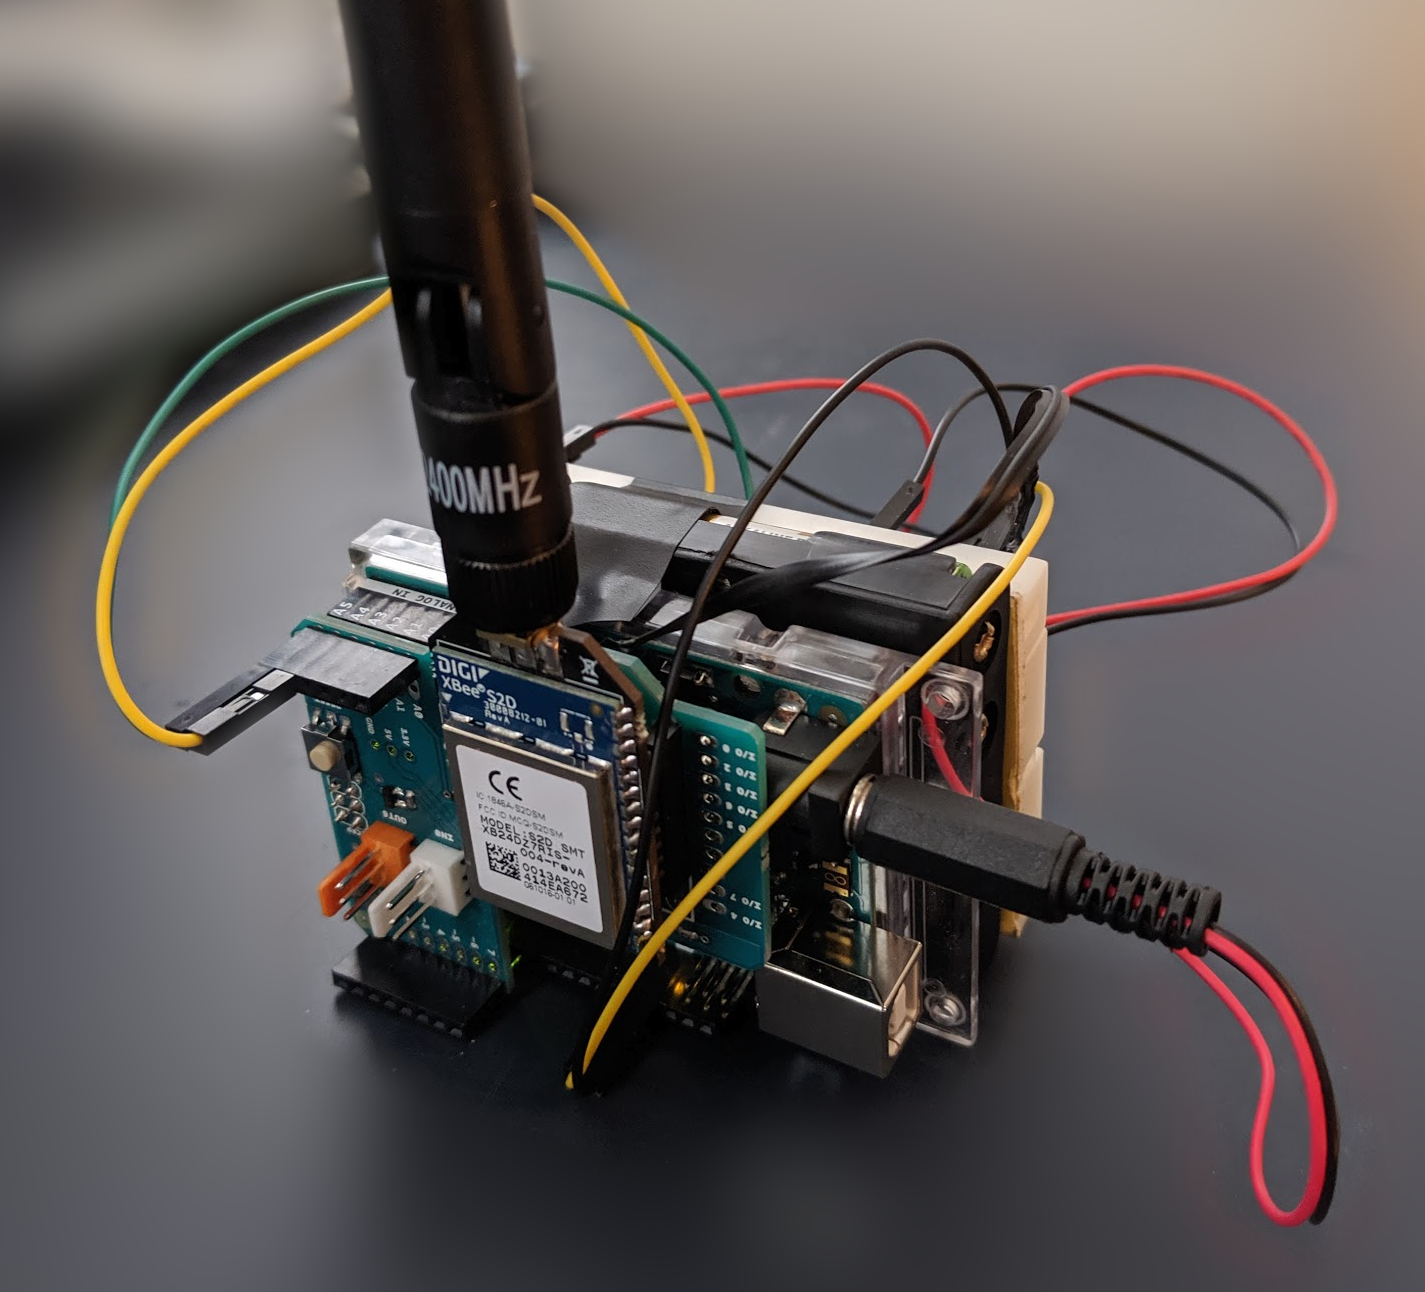
\includegraphics[width=10cm]{hardware}
    \caption{A node of the network.}
    \label{fig:node}
\end{figure}

\subsection{Arduino Uno}
Arduino Uno is a monothread microcontroller board based on the ATmega328P. It is able to use serial communication throw either USB or pins. Unfortunately, there's no possibilities to establish multiple connections and this may represent a limit (and in fact the project realization had to deal with that). The board comes also with 14 digital i/o pins and 6 analog pins.

\subsection{XBee Module}
The XBee Module is the device which allows different Arduino nodes to communicate wirelessly. The module is not able to send or receive data by itself and can only forward over-the-air data coming from the serial communication with a smart device. Other devices, equipped with XBee as well, will be able to receive and read the stream of data. The communication is based on modulation of waves in the electromagnetic spectrum.

\subsection{DHT22 temperature and humidity sensor}
The DHT22 sensor is well-known and widely used in this kind of projects. It can provide two different measurements and is more accurate than is predecessor DHT11. In fact, the temperature range which can be detected goes from -40 to 125\, \celsius\ with an accuracy of 0.5\, \celsius; the umidity index is provided as a percentage (0-100 \%) and the accuracy is 2-5 \%. It has been decided to poll the sensor each 2 seconds dues to the low sampling rate, which is 0.5 Hz. Even if it's better then the DHT11, this sensor is still not so accurate and responsive but sufficient for the project scope. 

\subsection{MMA8451 triple axis accelerometer}
The MMA8451 is a small accelerometer able to analyze three axis with a resolution of 14 bit. The maximum refresh rate can reach up to 800 Hz with a precision of approx. 1 / 10 000 g. The device comes with some embedded functions which can be customized by the developer: the most interesting one is the possibility to change between the normal polling mode and the interrupt one. In the first one, data is detected whenever explicitly required while in the second one, an interrupt is generated when movement is detected. The accelerometer communicate using I\textsuperscript{2}C digital output interface. In the proposed project, the device is queried each 250 ms.

\section{Software}
This section describes the software projects developed during the project starting from the node and going through to the user interface.

\subsection{Sensor}
The sensors themselves have been developed in C++ using the Arduino SDK. Contiki has been ruled out as a potential operating system given the last Arduino Contiki port is based on Contiki 2.2, which would have caused a lot of work just to get the sensors working on it.

The following defines can be used to customize the behavior of the sensor nodes:

\begin{description}
\item[SERIAL\_DEBUG] Disables ZigBee and uses the UART port as a debugging and logging interface instead (see sub section~\ref{subsec:uart}). This is helpful during development and for testing the sensors.
\item[ENABLE\_SECURITY] Enables the use of the security layer (see section~\ref{sec:security}). This causes much longer startup times due to potential issues with entropy generation (see sub section~\ref{subsec:entropy}).
\item[ZIGBEE\_RETRY] Enables a package retry logic for sending data packets. This can cause some delays if a sensor with a high output data rate is connected.
\end{description}

The sensor project has been implemented using the \href{https://platformio.org/}{PlatformIO development platform}. This IDE supports over 700 embedded platforms and relies on Visual Studio Code for the editor and code completion. It also manages the binary upload and supports logging through the serial port. The built in library manager gives simple access to thousands of open source libraries, most of them supporting the Arduino platform. It also restores these libraries from the internet when needed so it can be excluded from the source repository.

During the node lifetime it goes through multiple states:

\subsubsection*{Initialization state}
After booting up, the node starts with the initialization logic. During this time, it will:

\begin{itemize}
\item Check whether a temperature / humidity sensor is connected on PIN 13 and configure the mode accordingly
\item Initialize the I\textsuperscript{2}C bus on the analog inputs A4 and A5
\item Configure the accelerometer in 2G / high accuracy mode
\item Load / generate an ECC keypair and generate a nonce
\end{itemize}

\subsubsection*{Handshake state}
The handshake state will repeat every 5s until it succeeds. It will send a key handshake message to the server and wait for a reply back from it. Details of the handshake protocols are specified in section \ref{sec:security}.

\subsubsection*{Measurement state}
During this mode the sensor will read all available sensors and send the data to the server. If the retry logic is enabled it will also check for any transmission reports and discard / retry any sent packets. This is repeated every 250ms (2000ms if accelerometer is unavailable) to allow the device to go to sleep to conserve power.

If the transmission fails for more than 10s the node goes back into the handshake state.

\subsection{Router}\label{subsec:router}
The router is implemented in Python using the digi-xbee and requests library. It's only job is to connect to the coordinator (see section~\ref{sec:coordinator}) via the serial port and translate between ZigBee and the REST interface implemented in the dashboard (see sub section~\ref{subsec:api}).

\subsection{Dashboard}
All the data coming from sensors can be seen in different charts integrated into a fresh web dashboard. The realization of such interface rely on an open source project called \href{https://github.com/app-generator/flask-argon-dashboard}{Flask Argon Dashboard}, which is released under MIT License. Many functions can be found on this project: user authentication mechanisms and admin tools are just some examples in addition of a multitude of different template plots and graphs. For the aim of this project, all those tools were too much and the majority of them has been cut off in favor of a cleaner interface.

The decision of adopting this dashboard comes from how the interface itself has been developed: since is coded in \href{https://palletsprojects.com/p/flask/}{Python Flask} and well integrated with SQLite database and SQLAlchemy ORM (see \ref{subsec:database}), the setup it's been faster and more efficient since it was aligned with the design decisions that has been taken at the early stages of the project discussion.

After the graphical adjustments of the dashboard, API development (see \ref{subsec:api}) and charts creation has been the only missing pieces in order to get the final result. As already integrated by Argon Dashboard, charts are based on the famous \href{https://www.chartjs.org/}{Chart.js}, which has been properly adjusted in order to visualize in the more effective way data coming from different sensors (using different colors) and multi-axix (for humidity and temperature sensor).

\subsection{Database}\label{subsec:database}
Since SQLite and SQLAlchemy has always been a winning couple when associated with Python Flask, the triad has been chosen.
\href{https://www.sqlalchemy.org/}{SQLAlchemy} is an Object Relational Mapper which permit to handle in a more flexible and comprehensive way database, creating a sort of abstraction level in between the web server and the database itself. \href{https://www.sqlite.org/index.html}{SQLite} has been the easier, effective and fast open source SQL database engine which works perfectly together with SQLAlchemy.

The database structure has been divided into two different tables: the first one is the \textbf{Node} table, where sensor serial number are associated with an internal ID, while in the second table (called \textbf{Measurement}) incoming stats are stored with timestamp, type of measurement and origin sensor.

\subsection{API}\label{subsec:api}
The dashboard implements the following Web API, accepting requests in JSON to the specified endpoints.

\subsubsection*{Register node}
Registers a sensor node in the database using the Xbee serial number as the unique identifier.

\texttt{POST /api/v1/node/register}

\subsubsection*{Request parameters}
\begin{description}
\item[serial] Xbee serial number in HEX (unique node identifier)
\end{description}

\subsubsection*{Response parameters}
No content.

\subsubsection*{Status codes}
\begin{description}
\item[204 No content] Registration successful
\item[400 Invalid request] Invalid key or duplicate serial number
\end{description}

\subsubsection{Store measurement}
Stores a measurement for a given node.

\subsubsection*{URL}
\texttt{POST /api/v1/measurement}

\subsubsection*{Request parameters}
\begin{description}
\item[serial] Xbee serial number
\item[type] Sensor type (uint8)
\item[value] Sensor value as float
\end{description}

\subsubsection*{Response parameters}
No content.

\subsubsection*{Status codes}
\begin{description}
\item[204 No content] Measurement recorded successful
\item[400 Invalid request] Invalid sensor type
\end{description}

\subsubsection{Read measurements}
Reads measurement for display in chart.

\subsubsection*{URL}
\texttt{GET /api/v1/measurement}

\subsubsection*{Request parameters}
\begin{description}
\item[token] Token used for paging (optional)
\end{description}

\subsubsection*{Response parameters}
\begin{description}
\item[data] All data since the last token (in arbitrary format)
\item[token] Token for the next call
\end{description}

\subsubsection*{Status codes}
\begin{description}
\item[200 OK] Measurements
\end{description}

\section{Security}\label{sec:security}
\subsection{Overview}
The security layer provides an end-to-end encrypted and authenticated message channel for all data messages. The implementation is custom and is based on ECC for public key cryptography and AES for data encryption. During the handshake phase all the shared secrets for the data encryption are established between the server and the sensors. Additionally, the ZigBee based encryption mode can be used as another layer of security.

\subsection{Setup and Handshake}
During the deployment the server's public key is written to the sensor nodes' flash memory acting as a trust anchor. While directly using this key does not allow us to change it if it were compromised, it does simplify the protocol a lot and is definitely suitable for the scope of the project. In a full deployment of such sensor nodes this weakness should however be solved by implementing a three-leg handshake with proper authentication of the server using an offline key as the signature.

The sensor first enters the key establishment phase, consisting of the following steps:
\begin{enumerate}
\item Generate ECC keypair using secp256k1 curve and store in EEPROM (only on first boot)
\item Calculate shared secret using \texttt{SHA256(ECDH(privateKey, serverKey))[:16]}
\item Generate 32bit nonce \texttt{cNonce}
\item Send \texttt{HELO(serialNr, publicKey, {cNonce})}
\item Server checks the node, stores the public key, generates the same shared secret and a nonce (\texttt{sNonce}) and replies with \texttt{HELO({sNonce})}
\item Both sides derive the DK and IV to use with \texttt{DK, IV = HMAC-SHA256(HK,
cNonce + sNonce + serial)}
\end{enumerate}

During the handshake, the encryption mode is AES-128 with ECB and a 0-IV. Since the nonces are only 32bit each and are purely random data this is secure. The encryption of the nonces is theoretically not necessary, but it's used to prevent a MITM from modifying the handshake, since the encrypted nonce is expected to be only 32bit in length and the rest of the block is padded with 0 bits.

\subsection{Data transmission}
All data packets are expected to be of the form \texttt{DATA(serialNr, packetIndex, \{ measurements \})} using AES-128 in CTR mode. The IV is XORed with \texttt{packetIndex << 16}, which achieves multiple goals:

\begin{itemize}
\item The use of a deterministic (yet non-repeated) IV ensures that the IV does not have to be sent to the server, thus saving 16 byte of data per packet
\item Shifting the packetIndex by 16 bytes leaves the lower 16 bytes for use in the CTR operation mode, guaranteeing that no two blocks have the same key stream
\end{itemize}

\part{Results}
% Simulation results (for simulation-based projects) and measurements (testbed-based projects).

\part{Implementation limitations and challenges}
\section{Hardware challenges}
\subsection{Sensors}\label{subsec:sensors}
During the project development one of the constant annoyances has been the acceleration sensor. Often times the sensor works correctly and flawlessly for minutes and suddenly stops working. Wiggling with the jumper cables or resistors seems to fix the issue in some cases, so it's not a software issue. However, given it uses the I\textsuperscript{2}C bus and has to be initialized correctly if the connection fails during the startup it will never start to work. This issue has caused a lot of frustrated reboots of the sensor nodes during the development and also the final demo.

\subsection{Arduino UNO platform}\label{subsec:uart}
The Arduino platform is great for any kind of prototyping of IoT projects. However, the chosen board configuration for this project only has a single UART. Given XBee uses this port for its combination the situation arises where one constantly has to disconnect the modem to be able to upload a new version, put it back on and reconnect the power. Additionally debug logging is impossible until the network is working correctly and a remote logging facility has been implemented.

\subsection{Entropy generation}\label{subsec:entropy}
Generating entropy on embedded systems is never an easy task. The implementation we picked as an entropy source uses the lowest bit from the ADC of an unconnected analog PIN. This however can lead to very long times if more than a few bits of random data are required. In our case, the first device boot generating the encryption key could take up to a multiple minutes without any user feedback.

\end{document}
